\documentclass[a4paper,10pt]{article}
\usepackage[left=2cm, right=2cm, top=1cm, bottom=2cm]{geometry}
\usepackage{enumitem, hyperref}
\usepackage{fontawesome5}
\usepackage{tabularx}
\usepackage{ltablex}
\usepackage{tikz}
\usepackage{graphicx}
\usepackage{lmodern, titlesec}
\usepackage{parskip}
\usepackage{bold-extra}  % Enables bold small caps
\usepackage{tcolorbox}
\usepackage{ebgaramond}
\usepackage{soul}
\usepackage{xcolor}

% Tikz Libraries
\usetikzlibrary{mindmap,shadows,shadings}

% Define colors
\definecolor{burnt}{HTML}{913b01}
\definecolor{tealshade}{HTML}{bfdfdf}
\definecolor{burntshade}{HTML}{FFE0CF}

\titleformat{\section}
{\Large\bfseries\scshape\color{burnt}}  % Bold + Small Caps + Teal
{} % No numbering
{0pt} % No spacing
{} % No title prefix
[\vspace{0.1cm} \titlerule] % Adds spacing & horizontal rule

\keepXColumns

\renewcommand{\baselinestretch}{1.1}
\renewcommand{\labelitemi}{\textbullet}

\newcommand{\refnum}[2]{\href{#1}{\textbf{[#2]}}}

\hypersetup{
	colorlinks=true,
	linkcolor=teal,
	filecolor=teal,
	urlcolor=teal,
	citecolor=teal
}

\begin{document}
\begin{center}
	{\Huge\textbf{\href{https://henribranken.github.io/MyCV/}{\faHandPointer~ \textsc{Henri Branken}}}}\\[0.5cm]
\end{center}
\begin{minipage}{0.7\textwidth}
	% === Contact Information in a Styled Box ===
	\begin{tcolorbox}[
		colback=teal!10, % Light gray background
		colframe=teal,   % Teal border
		boxrule=1pt, % Border thickness
		width=0.8\textwidth,
		left=10pt, right=10pt, % Padding inside the box
		sharp corners=northwest
		]
		\begin{tabularx}{\textwidth}{c X}
			\faHome & \textbf{Potchefstroom (2531)} \\[0.2cm]
			\faEnvelope & \href{mailto:henri.branken777@gmail.com}{\textbf{henri.branken777@gmail.com}} \\[0.2cm]
			\faPhone & \textbf{+27 (0) 82 785 5983} \\[0.2cm]
			\faGithub & \href{https://github.com/HenriBranken}{\textbf{GitHub}} \\[0.2cm]
			\faLinkedin & \href{https://www.linkedin.com/in/henri-branken-1423a2153/}{\textbf{LinkedIn}}
		\end{tabularx}
	\end{tcolorbox}
\end{minipage}
\hfill
\begin{minipage}{0.3\textwidth}
	\begin{tikzpicture}
		% Shadow for depth
		\shade[ball color=tealshade, inner color=tealshade, outer color=tealshade, draw=teal] (0.2,-0.2) circle (2.3cm);
		
		% Circular clip for the image
		\clip (0,0) circle (2.3cm);
		\node[anchor=center] at (0,0) {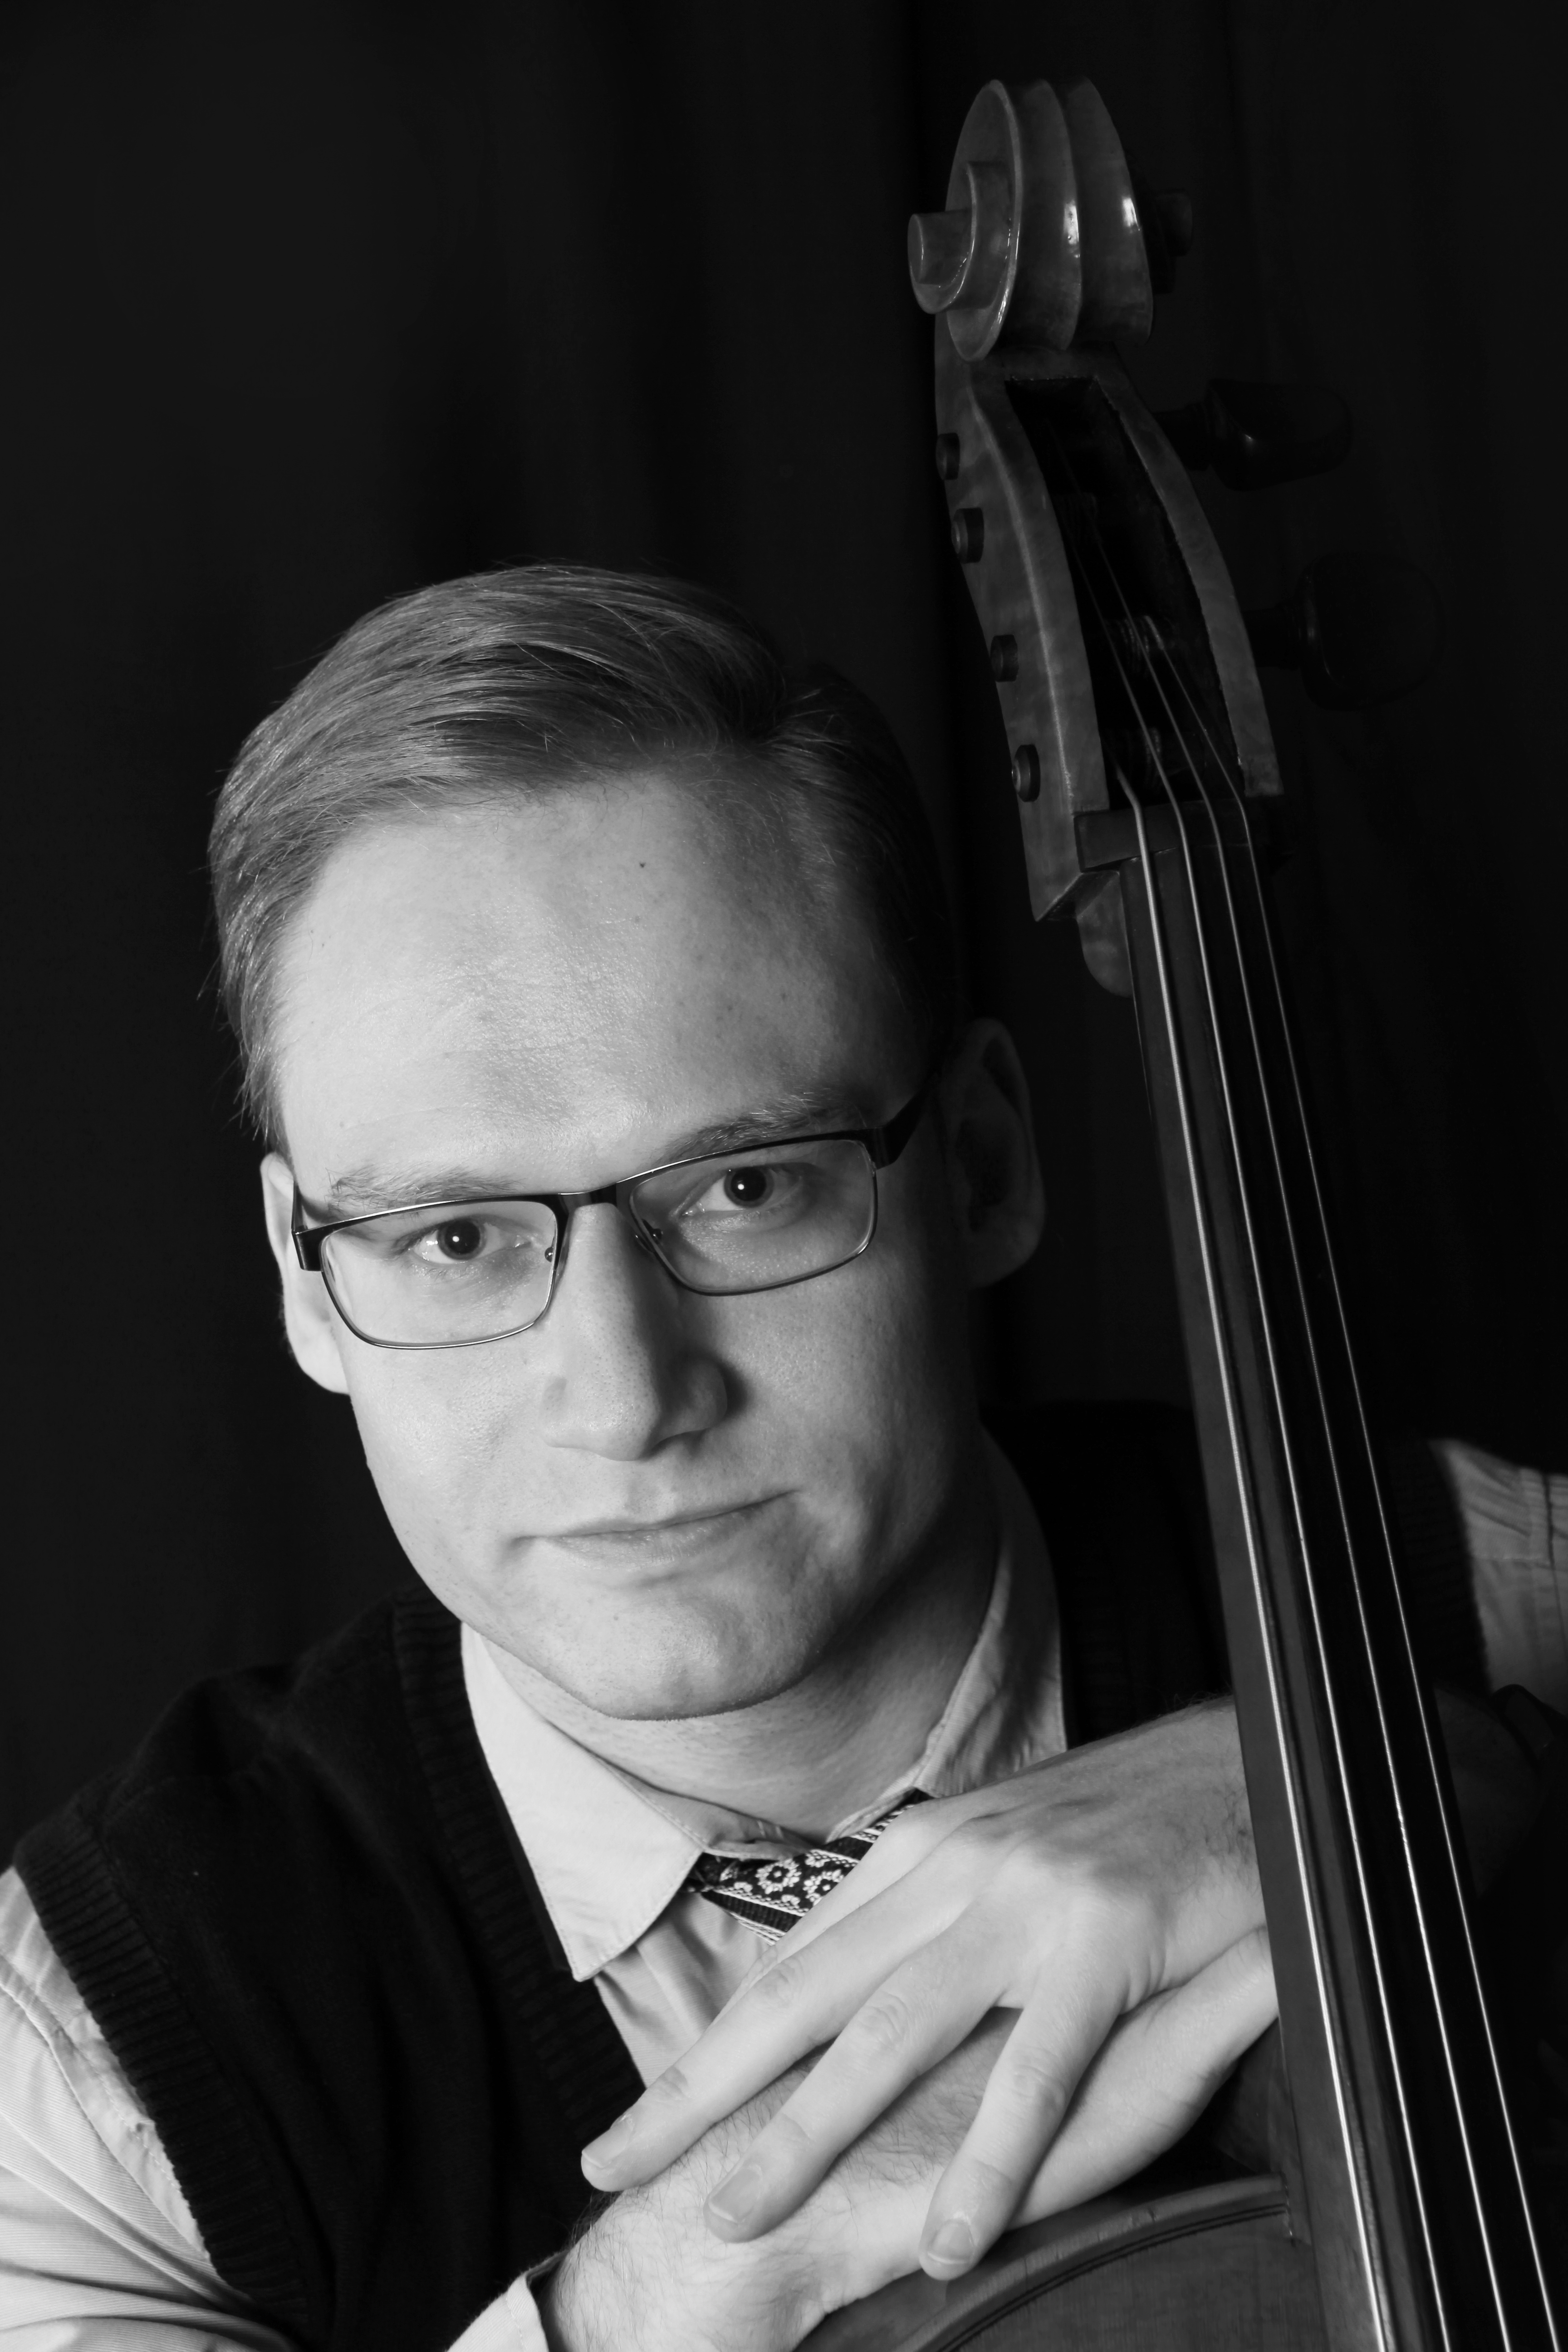
\includegraphics[width=4.6cm]{cello_11a}};
	\end{tikzpicture}
\end{minipage}\\[0.5cm]

% === Career Objective Box ===
\begin{tcolorbox}[
	colback=burntshade,    % Light teal background
	colframe=burnt,     % Burnt orange border
	boxrule=1pt,        % Border thickness
	sharp corners=northwest,
	rounded corners=southwest,
	coltitle=white,     % White title color
	fonttitle=\large\bfseries\scshape,  % Bold Small Caps title
	title=Career Objective,
	width=\textwidth,   % Full width
	left=10pt, right=10pt, top=5pt, bottom=5pt  % Padding inside the box
	]
	Seeking opportunities in \textbf{Web Development}, \textbf{Data Science}, \textbf{SQL Development}, or \textbf{Academic Mentoring} in Math, Science, and Programming to apply my technical skills and support learning.
\end{tcolorbox}

\section*{Overview}
I hold a Master's Degree in Space Physics (Cum Laude), which has equipped me with strong research capabilities and proficiency in mathematical analysis and modeling. Transitioning from academia, I gained approximately 3.5 years of experience as a Data Scientist at Matogen Applied Insights. There, I developed solutions such as a Portfolio Performance Monitor and Credit Loss Model for a telecommunications company, a PowerBI dashboard for monitoring agricultural nutrient distributions, and an AI model to predict grape harvesting dates.

To broaden my skillset, I completed a HyperionDev Bootcamp, mastering several programming languages including HTML, CSS, JavaScript, the MERN stack, and Java. This experience enhanced my understanding of full-stack web development and effective database management. Upon completion, I served as a Coding Mentor from July 2024 to the present time.

In summary, I have a strong scientific background, a deep interest in programming, and a naturally curious nature. While I can navigate Windows environments, I prefer working with Linux systems {\faLinux}
\section*{Languages}
\begin{itemize}
	\item \textsc{\textbf{Afrikaans}}: Mother Tongue
	\item \textsc{\textbf{English}}: Fluent, Level 5 TEFL Certification
\end{itemize}

\section*{Education and Training}
\renewcommand{\arraystretch}{1.1}
\begin{tabularx}{\textwidth}{r l X}
	\textbf{2024/07--2025/03} & \multicolumn{2}{| l}{\textbf{\href{https://www.hyperiondev.com/}{HyperionDev}} Code Reviewer \& Student Mentor} \\
	& \multicolumn{1}{| l}{\textbullet} & As a Coding Mentor, I evaluated students' coding submissions for tasks and provided constructive feedback to enhance the quality, efficiency, and styling of their code. Additionally, I conducted live sessions to provide personalised guidance, helping students effectively tackle specific tasks and develop their programming skills. \\
	& \multicolumn{1}{| l}{\textbullet} & Acted as an SME to refactor \href{https://github.com/HenriBranken/AcademicPortfolio/blob/main/Testing\_a\_React\_App.pdf}{\textbf{Task Contents}} for the course syllabus.\\
	& \multicolumn{1}{|l}{\textbullet} & Conducted an \href{https://github.com/HenriBranken/AcademicPortfolio/blob/main/Academic\%20Onboarding\%20Session.pdf}{\textbf{onboarding session}} for newly-enrolled students on the \href{https://livestorm.co/}{\textbf{LiveStorm}} platform. \\
	& \multicolumn{1}{|l}{\textbullet} & Please see my full Academic Portfolio \href{https://github.com/HenriBranken/AcademicPortfolio?tab=readme-ov-file\#academic-portfolio}{\textbf{here}}. \\
	& & \\[-5pt]
	
	\textbf{2023/01--2023/09} & \multicolumn{2}{| l}{\textbf{\href{https://www.hyperiondev.com/bootcamps/immersive/full-stack-web-and-software-engineer/}{HyperionDev Full Stack Web \& Software Engineer Bootcamp}}}\\
	& \multicolumn{1}{| l}{\textbullet} & HyperionDev is accredited with the \textbf{\href{https://www.mict.org.za/}{MICT Seta}} (ACC/2017/05/0005). This course bears \textbf{30 Credits}, aligned to an \textbf{NQF Level 5 Qualification}. \\
	& \multicolumn{1}{| l}{\textbullet} & Please click on this \href{https://www.hyperiondev.com/portfolio/79331/}{\textbf{link}} to view my entire HyperionDev Profile.\\
	& \multicolumn{1}{| l}{\textbullet} & I received a \href{https://www.facebook.com/henri.branken.9/posts/pfbid02gUh1H3ovPTfn4TLrr3ZYFWzhcEyuDte2xsZTLbPjHiNZStTRPEArNnius6T5Bj5rl}{\textbf{``Student of the Month'' Award}} for my commitment to excellence and continuous improvement.\\
	& \multicolumn{1}{| l}{\textbullet} & \textbf{Noteworthy GitHub Repos:} \refnum{https://github.com/HenriBranken/react\_hangman\#hangman-game-in-react}{1} Hangman Game (React UI). \refnum{https://github.com/HenriBranken/ReactDictionaryUsage\#dictionary-app}{2} Dictionary App (Interacting with 3rd-Party API). \refnum{https://github.com/HenriBranken/github\_app\#github-web-app}{3} GitHub API App (Express, React, Axios). \refnum{https://github.com/HenriBranken/CoolTech\#cooltech-credential-management-system}{4} Credential Management System (Authentication, Authorization). \refnum{https://github.com/HenriBranken/FoodQuick\#food-ordering-program-capstone}{5} Delivery App (Java OOP). \refnum{https://github.com/HenriBranken/PoisePMS\#poise-project-management-system-pms}{6} Project Management System (Java, JDBC, MySQL). \refnum{https://github.com/HenriBranken/ISS\#international-space-station-iss}{7} International Space Station (Asynchronous JavaScript). \refnum{https://github.com/HenriBranken/montyHall\#the-monty-hall-problem}{8} Monty Hall Game (React, State Management) \\
	& & \\[-5pt]
		
	\textbf{2022/08--2022/12} & \multicolumn{1}{| l}{\textbullet} &
	\textbf{\href{https://github.com/HenriBranken/Henri_Branken_Certification/blob/master/online_courses/TEFL_Certificate.pdf}{Qualifi Level 5 Diploma in Teaching English as a Foreign Language (The TEFL Academy)}} \\
	& \multicolumn{1}{| l}{\textbullet} & \href{https://github.com/HenriBranken/Henri_Branken_Certification/blob/master/online_courses/TEFL_20hour_certificate.pdf}{\textbf{Classroom TEFL Course Certificate (20 Hours)}} \\
	& \multicolumn{1}{| l}{\textbullet} & TEFL, Teaching Business English (30 Hours) \\
	& \multicolumn{1}{| l}{\textbullet} & The completion of my own \href{https://drive.google.com/file/d/1tkuLPdXlgsDundxbjZLjyl6aZhKUqDid/view?usp=sharing}{\textbf{Japanese Language Studies book}} (typeset in \href{https://en.wikipedia.org/wiki/LaTeX}{\textbf{\LaTeX}}), which took 4+ years. Without a doubt, this is the project I’m most proud of! \\
	& & \\[-5pt]
	
	\textbf{2019--2022/07} & \multicolumn{2}{| X}{\textbf{Data Scientist at \href{https://ai.matogen.com/}{Matogen Applied Insights}}} \\
	& \multicolumn{1}{| l}{\textbullet} & Built PowerBI Dashboard to monitor Nutrient Distributions of Farm Crops.\\
	& \multicolumn{1}{| l}{\textbullet} & Built Tableau Dashboards for a Debt Counseling Company to closely track agent performance.\\
	& \multicolumn{1}{| l}{\textbullet} & Interrogated the \href{https://hcup-us.ahrq.gov/nisoverview.jsp}{\textbf{Nationwide Inpatient Sample (NIS)}} to determine factors influencing mortality rates in patients receiving orthopedic procedures.\\
	& \multicolumn{1}{| l}{\textbullet} & Built an AI Model to improve the accuracy of harvest-date predictions for grape cultivars.\\
	& \multicolumn{1}{| l}{\textbullet} & Built a Portfolio Performance Monitor and Expected Credit Loss Model for a Telco Company based on Service Line Age Files and Bureau Data.  Here are \href{https://github.com/henri-branken-matogen/henri_libs}{\textbf{PySpark Libraries}} I translated from SAS.\\
	& \multicolumn{1}{| l}{\textbullet} & Made a \href{https://github.com/HenriBranken/ProbeSchedule}{\textbf{Python Algorithm}} to compute accurate Water Irrigation Schedules for Farm Crops based on telemetry readings and weather forecasts.  This was to improve on the crude method of setting water irrigation parameters based on season of the year.\\
	& & \\[-5pt]
	
	\textbf{2018} & \multicolumn{1}{| l}{\textbullet} & Completed \href{https://github.com/HenriBranken/Henri\_Branken\_Certification?tab=readme-ov-file\#online-courses-completed-at-datacamp-in-alphabetical-order}{\textbf{Online Courses}}
	 at \textbf{\href{https://www.udemy.com/}{Udemy}} and \textbf{\href{https://www.datacamp.com/}{DataCamp}} with a strong focus on \textbf{Python Data Science} and \textbf{Linux Essentials}. \\
	& \multicolumn{1}{| l}{\textbullet} & Attended \textbf{\href{https://2018.za.pycon.org/}{PyConZA 2018}} in Johannesburg.\\
	& & \\[-5pt]
	
	\textbf{2017} & \multicolumn{1}{| l}{\textbullet} &
	Internship at the \href{https://natural-sciences.nwu.ac.za/space-research}{\textbf{Centre for Space Research, Potchefstroom}} \\
	& \multicolumn{1}{| l}{\textbullet} & Completed the \textbf{``Data Science with Python'' Track} on \href{https://www.datacamp.com/}{\textbf{DataCamp}} \href{https://www.datacamp.com/Certificate\#13,897}{\textbf{(Certificate Number \#13,897)}}.\\
	& \multicolumn{1}{| l}{\textbullet} & Completed the 2017 \textbf{\href{https://adventofcode.com/}{Advent of Code}} challenges. My Python solutions may be viewed in this \href{https://github.com/HenriBranken/Advent_of_Code_2017_python_3}{\textbf{repo.}} \\
	& & \\[-5pt]
	
	\textbf{2014--2016} & \multicolumn{2}{| X}{\textbf{Master of Science in \textsc{Space Physics}, \href{https://www.nwu.ac.za/}{North-West University}, Potchefstroom}}\\
	& \multicolumn{2}{| X}{\textsc{Dissertation:} \href{https://repository.nwu.ac.za/handle/10394/25063}{\textit{\textbf{Weighing dark matter in brightest cluster galaxies}}}}\\
	& \multicolumn{2}{| X}{\textsc{Supervisor:} Prof. Ilani Loubser} \\
	& \multicolumn{2}{| X}{\textsc{Avg. Score:} 85\%, \textit{Cum Laude}} \\
	& \multicolumn{2}{| X}{Awarded as the top achiever on Master’s level in the Centre for Space Research (for the year 2016).} \\
	& \multicolumn{2}{| X}{\href{https://github.com/HenriBranken/Henri_Branken_Certification/blob/master/tertiary/full_university_academic_record.pdf}{\textbf{Academic Transcript}}} \\
	& & \\[-5pt]

	\textbf{2013} & \multicolumn{2}{| X}{\textbf{Honours Bachelor of Science in \textsc{Physics}, \href{https://www.nwu.ac.za/}{North-West University}, Potchefstroom}}\\
	& \multicolumn{2}{| X}{\textsc{Avg. Score:} 92\%, \textit{Cum Laude}}\\
	& \multicolumn{2}{| X}{Awarded as the Top Achiever in Honours in Physics.}\\
	& & \\[-5pt]

	\textbf{2010--2012} & \multicolumn{2}{| X}{\textbf{Bachelor of Science in \textsc{Physical and Chemical Sciences}, \href{https://www.nwu.ac.za/}{North-West University}, Potchefstroom}} \\
 	& \multicolumn{2}{| X}{Majored in \textbf{Physics and Applied Mathematics}} \\
 	& \multicolumn{2}{| X}{\textsc{3rd Year Avg. Score:} 95\%, \textit{Cum Laude}} \\
 	& \multicolumn{1}{| l}{\textbullet} & Awarded as the top achiever in the 1\textsuperscript{st}, 2\textsuperscript{nd}, and 3\textsuperscript{rd} years of the Physics curriculum.\\
	& \multicolumn{1}{| l}{\textbullet} & Awarded as the top student in the Faculty of Natural Sciences for the 1\textsuperscript{st} and 3\textsuperscript{rd} years of study.\\
	& \multicolumn{1}{| l}{\textbullet} & \href{https://github.com/HenriBranken/Henri_Branken_Certification/blob/master/tertiary/Supplemental_Instruction_Leader.pdf}{\textbf{Supplemental Instruction Leader}} for the 2011 Term in Mathematics (1\textsuperscript{st} year level).\\
	& & \\[-5pt]

	\textbf{2009} & \multicolumn{2}{| X}{\textbf{Matriculated with 8 distinctions from St. Andrew’s Private School, Welkom}}\\
	& \multicolumn{2}{| X}{\textbf{Avg. Score:} 89\%, \textit{With Distinction}}\\
\end{tabularx}

\begin{center}
\tikz[mindmap, text=white, grow cyclic, concept color=burnt, font=\Large\bfseries,
root concept/.append style={
	minimum size=2.5cm
},
level 1 concept/.append style={
	sibling angle=90,
	level distance=5cm,
	every child/.style={concept color=teal, font=\bfseries}
},
level 2 concept/.append style={
	sibling angle=45,
	level distance=3cm,
	every child/.style={concept color=tealshade, text=black}
}]
\node [concept] {Henri's Experience}
child {node [concept] {Full-Stack \\ Web Dev}
	child {node [concept] {PHP}}
	child {node [concept] {Java}}
	child {node [concept] {jQuery}}
	child {node [concept] {MERN}}
	child {node [concept] {HTML, CSS, \\ JavaScript}}
}
child {node [concept] {Data Science}
	child {node [concept] {EDA, Data Wrangling}}
	child {node [concept] {PowerBI, Tableau}}
	child {node [concept] {Linux, BASH}}
	child {node [concept] {Git CLI, GitHub}}
	child {node [concept] {Pandas, NumPy, SciPy}}
	child {node [concept] {DataBricks, \\ SnowFlake, SQL, PySpark}}
	child {node [concept] {Python, \\ Jupyter Notebook}}
}
child {node [concept] {Research}
	child {node [concept] {\LaTeX, TikZ}}
	child {node [concept] {Maths}}
	child {node [concept] {Physics, Astrophysics}}
	child {node [concept] {LibreOffice Suite}}
	child {node [concept] {ChatGPT}}
}
child {node [concept] {Teaching}
	child {node [concept] {Qualify \\ Level 5 \\ Diploma}}
	child {node [concept] {Teaching \\ Business \\ English}}
	child {node [concept, minimum size=2.2cm] {HyperionDev Code Reviewer}}
	child {node [concept, minimum size=2.2cm] {HyperionDev \\ Coding Mentor}}
};
\end{center}

\section*{References}
	\begin{tabularx}{\textwidth}{l X}
	\textbf{Lauren Berrington} & HyperionDev, Previous Head of Education Operations \\
	& \faEnvelope \quad \href{mailto:laurenberrington@gmail.com}{\textbf{laurenberrington@gmail.com}} \\[0.1cm]
		
	\textbf{Seraaj De Villiers} & HyperionDev, Technical Education Manager \\
	& \faEnvelope \quad \href{mailto:seraajd@hyperiondev.com}{\textbf{seraajd@hyperiondev.com}} \\[0.1cm]
	
	\textbf{Prof. Christo Venter} & North-West University, Astrophysics Professor \\
	& \faEnvelope \quad \href{mailto:christo.venter@nwu.ac.za}{\textbf{christo.venter@nwu.ac.za}} \\[0.1cm]
	
	\textbf{Mr. Jacobus Eksteen} & CEO, Matogen Applied Insights \\
	& \faEnvelope \quad \href{mailto:jacobus.eksteen@ai.matogen.com}{\textbf{jacobus.eksteen@ai.matogen.com}} \\[0.1cm]
	
	\textbf{Mr. Bayan Dekker} & Former CEO, BluNova\\
	& \faEnvelope \quad \href{mailto:bayand@versuro.com}{\textbf{bayand@versuro.com}} \\[0.1cm]
	
	\textbf{Mrs. Tina Marx} & Data Architect, Matogen Applied Insights\\
	& \faEnvelope \quad \href{mailto:tina.marx@ai.matogen.com}{\textbf{tina.marx@ai.matogen.com}} \\[0.1cm]
\end{tabularx}
	
\end{document}